

\section{User Study}

We conducted a user study in order to evaluate the accuracy whether our hypothesis was true or not.

......

\subsection{Method}

We divided users into two groups by whether they have the same native language or not. So there are native language and foreign language group respectively. Foreign language group are required to use their native language to communicate with each other. About our experiment, every team will have two players and be placed in two different room. Players play Mote Robot with each other through Internet connection. Totally we tested 24 groups with 48 users, inclusive of 12 native language groups and 12 foreign language groups.

In our experiment, we provided three different types of communication manners to play Mute Robot:
\begin{enumerate}
    \item Speaking: 
    Traditional gameplay manner, user can communicate through speaking language.
    \item Body Language: 
    players can communicate through body language.
    \item using Speaking and Body Language together: 
    players can communicate with each other through speaking language and body language.
\end{enumerate}

In order to eliminate order effects, each user played Mute Robot with counterbalance by administering the various types of game in different sequence. After playing each type of Mute Robot, players will fill out an eSFQ\cite{eSFQ} questionnaire to evaluate gameplay experience. Besides, When players finished all three types of Mute Robot, they will need to fill out another final questionnaire and proceed user interview. It needs about 1 hour to finish our user study experiment. We would conduct video recording at all experiment process and used these video to do CPMs\cite{CPMS} (see Figure~\ref{fig:US1}). , which used to evaluate user gameplay experience.

\begin{figure}[!h]
\centering
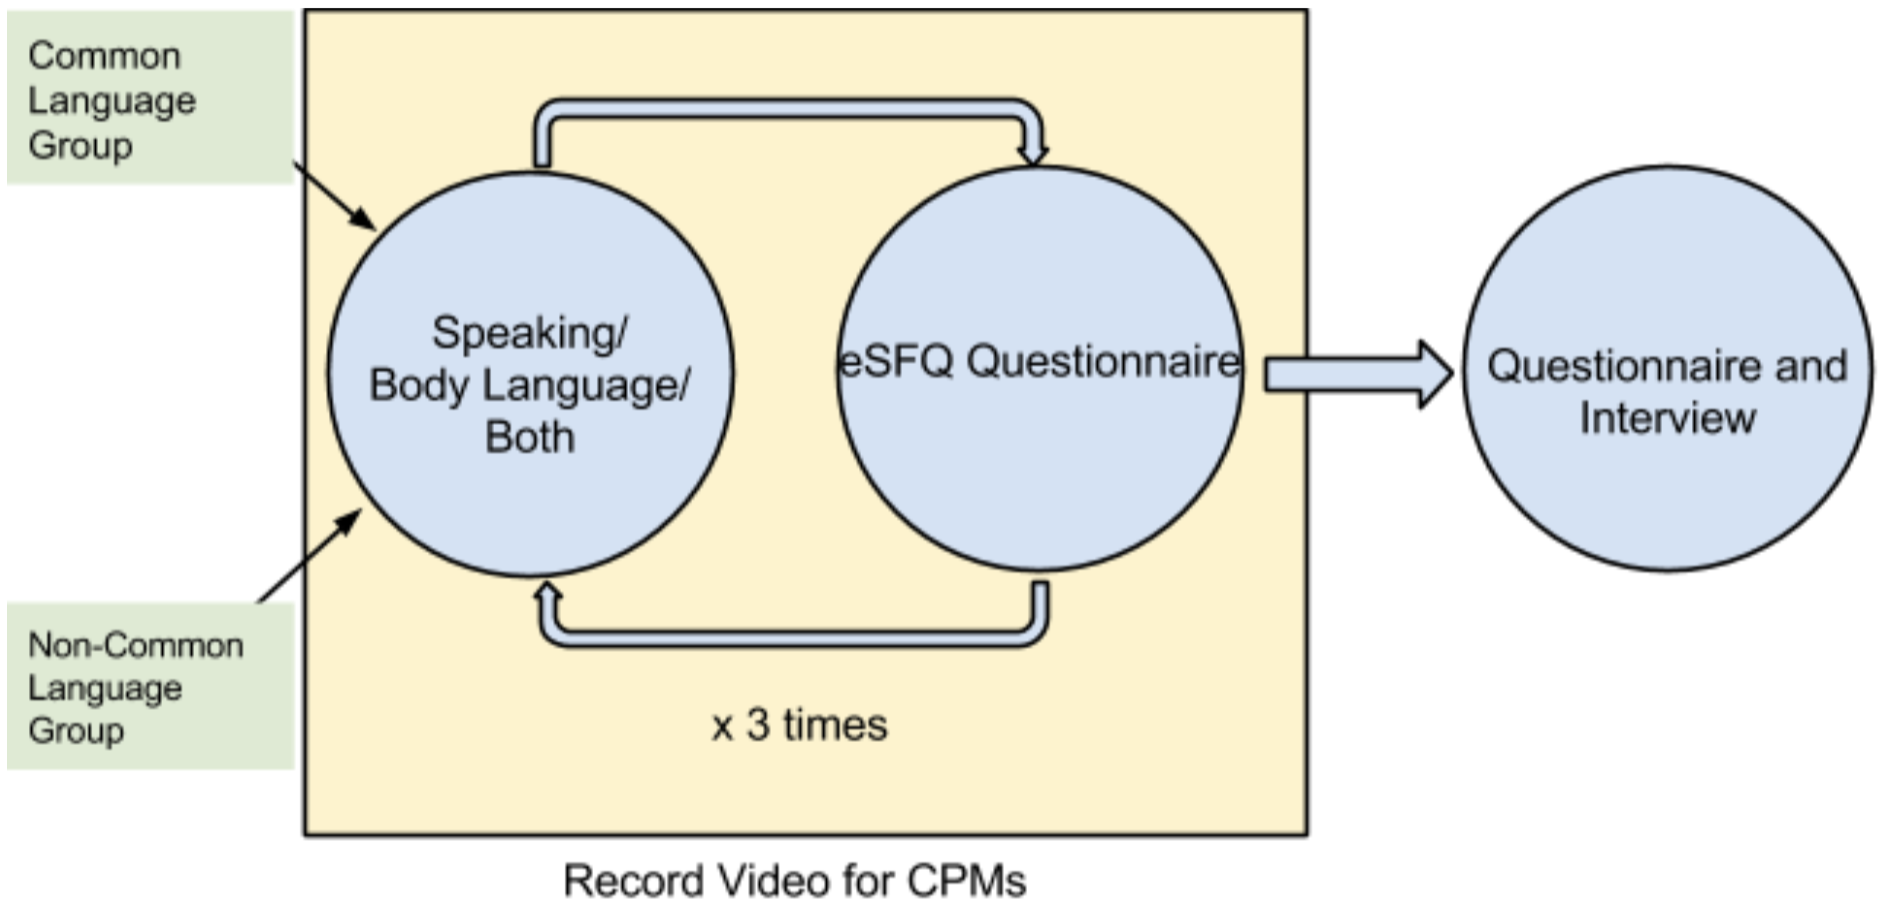
\includegraphics[width=0.9\columnwidth]{Figures/US_F1.png}
\caption{?????????}
\label{fig:US1}
\end{figure}



\subsubsection{Process}

\subsection{Observation}

\subsubsection{Communication Pattern}


\begin{table}[!h]
\renewcommand\arraystretch{1.5}
  \centering
  \begin{tabular}{
  !{\vrule width2pt}p{0.22\columnwidth}
  !{\vrule width2pt}p{0.08\columnwidth}
  !{\vrule width2pt}p{0.08\columnwidth}
  !{\vrule width2pt}p{0.08\columnwidth}
  !{\vrule width2pt}p{0.08\columnwidth}
  !{\vrule width2pt}p{0.08\columnwidth}
  !{\vrule width2pt}p{0.08\columnwidth}
  !{\vrule width2pt}}
    \Xhline{2pt}
    \multicolumn{1}
    {!{\vrule width2pt}c!{\vrule width2pt}}
    {\tabhead{\multirow{2}{*}{Inter-rater}}} &
    \multicolumn{6}
    {c!{\vrule width2pt}}
    {\centering\tabhead{Kappa for Metrics}} \\
    \Xcline{2-7}{2pt}
    % \hline
    & M1 & M2 & M3 & M4 & M5 & M6 \\
    \Xhline{2pt}
    Session1 & 0.75 & 1 & 0.79 & 1 & 1 & 1 \\
    \Xhline{2pt}
    Session2 & 1 & 0.8 & 1 & 1 & 1 & 1 \\
    \Xhline{2pt}
    Session3 & 0.75 & 1 & 0.87 & 1 & 1 & 1 \\
    \Xhline{2pt}
    Session4 & 1 & 1 & 0.96 & 1 & 1 & 1 \\
    \Xhline{2pt}
    Average & 0.88 & 1.2 & 0.91 & 1 & 1 & 1 \\
    \Xhline{2pt}
  \end{tabular}
  \caption{Inter-rater Agreement (M stands for CPM)}
  \label{tab:table2}
\end{table}


\subsection{Result}

% For common language group:
% The mean of the experienced fun level for “speaking” was 3.58(SD = x,xx) (5 meaning “Yeah, fun” – highest level of fun and 1 meaning “Yawn, boring” – lowest level of fun). 38\% of the users indicated that they wanted to play the game again, 58\% indicated maybe and only 4\% did not want to play again.Their game experiences were related to simple (83 \% of the users), and intuitive (54 \%). 
% The mean of the experienced fun level for “body language” was 4.54(SD = x,xx). 83\% of the users indicated that they wanted to play the game again, 13\% indicated maybe and only 4\% did not want to play again.Their game experiences were related to fun (79 \% of the users), intuitive (54 \%), exciting (46\%) and great (42 \%).
% The mean of the experienced fun level for “both” was 3.96(SD = x,xx). 63\% of the users indicated that they wanted to play the game again, 29\% indicated maybe and only 8\% did not want to play again.Their game experiences were related to fun (63 \% of the users), intuitive (63 \%), simple (63 \%) and exciting (33 \%).   

% For non-common language group:
% The mean of the experienced fun level for “speaking” was 4.08 (SD = x,xx). 54\% of the users indicated that they wanted to play the game again, 38\% indicated maybe and only 8\% did not want to play again.Their game experiences were related to fun (50 \% of the users), great (42 \%), intuitive (38 \%) ,simple (38 \%) and confusing (33 \%). 
% The mean of the experienced fun level for “body language” was 4.46(SD = x,xx). 75\% of the users indicated that they wanted to play the game again, 17\% indicated maybe and only 8\% did not want to play again.Their game experiences were related to fun (83 \% of the users), intuitive (54 \%), exciting (46 \%), simple (38 \%) and difficult (33 \%). 
% The mean of the experienced fun level for “both” was 4.5(SD = x,xx). 63\% of the users indicated that they wanted to play the game again, 37\% indicated maybe and no one did not want to play again.Their game experiences were related to fun (75 \% of the users), intuitive (67 \%), exciting (42 \%), simple (42 \%), great (34 \%) and confusing (33 \%). 
% (要改 強調難度)
% No matter common language or non-common language group,the fun/enjoyment rating of ”body language” and “both” were better than ”speaking”.Overall,”body language” got the best rating , and the rating for “both” only slightly lower but still very good, “speaking” got the worst rating. 
% For non-common language group , users thought speaking with different language was interesting and made this game harder,so the rating for “speaking” was better than common language group.And users feel confusing for “speaking” and “both”,在”body language”則沒有

\subsection{Discussion}


